\documentclass[letterpaper]{article}
\usepackage[submission]{aaai2026}
\usepackage{times}
\usepackage{helvet}
\usepackage{courier}
\usepackage[hyphens]{url}
\usepackage{graphicx}
\urlstyle{rm}
\def\UrlFont{\rm}
\usepackage{natbib}
\usepackage{caption}
\usepackage{xcolor}
\newcommand{\revE}[1]{\textcolor{red}{#1}}
\frenchspacing
\setlength{\pdfpagewidth}{8.5in}
\setlength{\pdfpageheight}{11in}
\pdfinfo{
/TemplateVersion (2026.1)
}
\setcounter{secnumdepth}{2}

\usepackage{algorithm}
\usepackage[noend]{algpseudocode}
\usepackage{amsmath}
\usepackage{amssymb}
\usepackage{longtable}
\usepackage{booktabs}
\usepackage{tikz}
\usepackage[capitalize,noabbrev]{cleveref}
\usetikzlibrary{positioning, fit, backgrounds, calc, decorations.pathreplacing}
\usepackage{multirow}

\title{Parallel Multiobjective Decision Diagrams} %TODO Please add

\author{
Rahul Patel\textsuperscript{},
Elias B. Khalil\textsuperscript{}
}
\affiliations{
Department of Mechanical and Industrial Engineering, University of Toronto, Canada\\
rm.patel@mail.utoronto.ca, elias.khalil@utoronto.ca
}

\newcommand{\mink}{\oplus}

\begin{document}

\maketitle

\begin{abstract}
Decision diagrams (DDs) can efficiently enumerate the exact Pareto frontier (PF) for multiobjective discrete optimization problems that admit a dynamic programming formulation.
The filtering of dominated labels at each node of the DD is a key step during enumeration. Its computational complexity grows quadratically with the cardinality of the intermediate label sets.
Furthermore, the filtering is performed serially by the existing algorithms, making it the primary bottleneck.
%The Pareto dominance filtering at each node of the DD has a cost that grows quadratically in the size of the intermediate labels. 
% Existing algorithms perform the filtering serially, leaving significant room for parallelization.
In this work, we propose a parallelization scheme for DD-based PF enumeration to address this challenge.
In particular, we propose \textsc{Pmdd} (Parallel Multiobjective Decision Diagrams), which not only parallelizes the dominance filtering but also the expansion, coupling and merging of label sets, tailored to both CPU and GPU.
We evaluate our methods on benchmark instances of the multiobjective knapsack, set packing, and traveling salesperson problems, comparing against state-of-the-art MIP and serial DD approaches.
We demonstrate that DD-based serial enumeration outperforms the MIP baseline in most cases.
Furthermore, our CPU parallel variants achieve speedups of up to $7.83\times$ while GPU variants reach up to $20.88\times$ relative to serial enumeration, when intermediate frontiers fit in GPU memory.
The code is available at \url{https://anonymous.4open.science/r/DD-C683/}.
\end{abstract}

\section{Introduction}
\label{sec:intro}

Many discrete optimization problems that arise in sustainability~\citep{flecker2022reducing}, finance~\citep{bonami2009exact}, healthcare~\citep{ehrgott2010mathematical}, routing~\citep{kovacs2015multi}, to name a few, are inherently multiobjective. In vehicle routing, for example, a dispatcher might need to balance the routing cost and service quality. As these goals conflict, no single plan is best in terms of cost and service quality at once. To compare different plans we use the principle of \emph{Pareto dominance}, where one solution dominates another if it matches it on every objective and improves on at least one. The goal of exact multiobjective optimization~\citep{ehrgott2005multicriteria,ehrgott2016exact,miettinen1999nonlinear} is to enumerate all nondominated solutions, i.e., the \emph{Pareto frontier} (PF), since each one represents a distinct trade-off a decision-maker might prefer over the rest. 

% In this work, we focus on multiobjective discrete optimization (MODO) problems with linear objectives and constraints. Exact methods for these problems are conventionally built on top of an integer linear programming (ILP) solver and fall into two families~\citep{halffmann2022exact}. \emph{Decision-space} methods search the space of feasible assignments, extending single-objective branch-and-bound with dominance-based pruning, i.e., a node is discarded only when its bound set is dominated by the incumbent frontier. Their performance therefore rests on the quality of the bound sets, and weak bounds translate directly into more branching. They are also vulnerable to symmetry. Equivalent partial assignments appear as distinct subproblems, and branch-and-bound re-explores each of them unless the symmetry is broken explicitly. \emph{Objective-space} methods search the image of the feasible set instead. They repeatedly solve scalarized single-objective ILPs restricted to a region of the objective space, remove the region dominated by each new nondominated point, and recurse on what remains. The ILP solver is a black box here, called once per region, so the number of independent NP-hard solves grows with the size of the frontier and, sharply, with the number of objectives. Many of these solves are redundant, returning an already known nondominated point or reporting infeasibility.

In this work, we consider multiobjective discrete optimization (MODO) problems with linear objectives and constraints. Exact methods are typically built on integer linear programming (ILP) solvers and fall into two families~\citep{halffmann2022exact}. \emph{Decision-space} methods extend single-objective branch-and-bound by pruning a node only when its bound set is dominated by the incumbent frontier. Their performance therefore depends critically on bound quality: weak bounds lead directly to additional branching. They are also susceptible to symmetry, since equivalent partial assignments are treated as distinct subproblems unless symmetry is explicitly broken. \emph{Objective-space} methods instead search the image of the feasible set. They repeatedly solve scalarized ILPs over restricted objective-space regions, remove regions dominated by newly discovered nondominated points, and recurse on the remainder. Because the ILP solver is invoked as a black box for each region, the number of independent NP-hard solves grows with the frontier size and, more sharply, with the number of objectives. Many such solves are redundant, either rediscovering known nondominated points or proving infeasibility.

Decision diagrams (DDs) have recently emerged as an effective framework for single-objective discrete optimization~\citep{bergman2016decision}. A DD is a layered acyclic graph that compactly represents the feasible set of a problem with a dynamic programming (DP) formulation. Layers correspond to decision variables, nodes to DP states, and arcs to variable assignments, yielding a one-to-one correspondence between feasible solutions and root-to-terminal paths. By merging partial assignments that reach the same DP state, DDs collapse symmetric and equivalent subproblems rather than re-exploring them.

% \citet{bergman2016multiobjective} extended the use of DDs to solve MODO problems. \citet{bergman2022network} further enhanced this method by incorporating advanced enumeration techniques and state-based label pruning operations. 
% However, a DD by itself, however, does not make PF enumeration cheap. Every node stores a nondominated set of labels for the partial paths that reach it. Expanding a layer generates new candidate labels along outgoing arcs, merges them into each destination node's frontier, and discards the ones some other label dominates. This dominance filtering is the dominant cost: in the worst case it compares every candidate at a node against every other candidate, and label sets grow quickly with the number of objectives. Enumeration also works inward from both ends of the diagram, alternating between expanding forward from the root and backward from the terminal until the two meet at a shared middle layer, the \emph{cutset}, where the root-side and terminal-side frontiers are combined and filtered once more. Existing DD-based MODO solvers perform all of this one node and one comparison at a time.

\citet{bergman2016multiobjective} extended DDs to MODO, and \citet{bergman2022network} strengthened the framework with improved enumeration and state-based label pruning. PF enumeration nevertheless remains expensive. Each node stores the nondominated labels of the partial paths reaching it. Layer expansion generates labels along outgoing arcs, merges them into destination frontiers, and removes dominated candidates. This dominance filtering is the main computational bottleneck: in the worst case, every candidate at a node is compared with every other, and label sets grow rapidly with the number of objectives. Enumeration proceeds from both ends of the diagram, alternating between forward expansion from the root and backward expansion from the terminal. The two searches meet at a middle layer, the \emph{cutset}, where their frontiers are combined and filtered again. Existing DD-based MODO solvers perform these operations sequentially, one node and one comparison at a time.
This paper investigates the parallelization of exact DD-based PF enumeration. 
% Although parallelism has been studied for single-objective DD search~\citep{bergman2014parallel,perez2018parallel,tardivo2024cp,tardivo2026gpu}, PF enumeration exposes distinct opportunities for parallelism because it processes large sets of labels rather than a single scalar value. 
% Computation can be parallelized across nodes during layer expansion, across labels during candidate generation and dominance filtering, and across nondominated sets during the final cutset merge. These levels of parallelism suit different architectures: multi-core CPUs support node-level work sharing and tree-based frontier reduction, while GPUs exploit finer-grained parallelism through flat candidate buffers and data-parallel filtering kernels.


% We make the following contributions:
% \begin{itemize}
%     \item We identify where bidirectional PF enumeration decomposes for parallel execution: across nodes within a layer, across labels within a node, and across products and merges in the coupling phase.
%     \item We build a CPU implementation that dynamically schedules node expansion over OpenMP threads and reduces cutset frontiers with a lock-free pairwise tree merge.
%     \item We develop a GPU implementation that flattens the diagram into offset-indexed arc arrays, expands each layer with a four-kernel pipeline, and merges the cutset in memory-bounded batches against a running frontier.
%     \item We evaluate on MOKP, MOSPP, and MOTSP instances with up to seven objectives against a state-of-the-art MIP baseline~\citep{dachert2024simple} and the state-of-the-art serial DD baseline~\citep{bergman2022network}, and show that our parallel CPU and GPU variants cut enumeration time relative to serial DD by up to $7.83\times$ and $20.88\times$ respectively, with the GPU fastest when frontiers fit in device memory and the CPU more reliable when they do not.
% \end{itemize}
We make the following contributions. We identify three sources of parallelism in bidirectional PF enumeration, namely node expansion within a layer, label processing within a node, and frontier products and merges during the coupling phase. We develop a CPU implementation that dynamically distributes node expansion across OpenMP threads and combines cutset frontiers using a lock-free pairwise reduction tree. We develop a GPU implementation that flattens the diagram into offset-indexed arc arrays, expands each layer with a four-kernel pipeline, and merges the cutset in memory-bounded batches against a running frontier. We evaluate the proposed methods on multiobjective variants of knapsack, set packing and traveling salesperson instances. We compare them with a state-of-the-art MIP method~\citep{dachert2024simple} and a state-of-the-art serial DD method~\citep{bergman2022network}. Relative to the serial DD method, the CPU and GPU implementations reduce enumeration time by up to $7.83\times$ and $20.88\times$, respectively. The GPU performs best when the frontiers fit in device memory, while the CPU is more robust when they do not.

% The remainder of this paper is organized as follows. \Cref{sec:prelim} provides background on MODO and DDs. \Cref{sec:method} describes the parallel enumeration methodology. \Cref{sec:results} presents the computational evaluation. \Cref{sec:related} reviews related work. \Cref{sec:conclusion} concludes the paper.

\section{Background}
\label{sec:prelim}
\subsection{Multiobjective Discrete Optimization}
\label{sec:prelim_modo}
A MODO problem can be defined as the minimization of an $m$-dimensional objective vector function $\mathbf{f}(\mathbf{x}) = (f_1(\mathbf{x}), f_2(\mathbf{x}), \dots, f_m(\mathbf{x}))^\top$ subject to $\mathbf{x} \in \mathcal{X}$. Here, $\mathbf{x} = (x_1, x_2, \dots, x_n)^\top$ represents a vector of discrete decision variables, and $\mathcal{X} \subseteq \mathbb{Z}^n$ is the bounded, discrete feasible region. We compare different feasible solutions based on the principle of \emph{Pareto dominance}. For any two feasible solutions $\mathbf{x}^1, \mathbf{x}^2 \in \mathcal{X}$, the solution $\mathbf{x}^1$ is said to Pareto dominate $\mathbf{x}^2$, denoted by $\mathbf{f}(\mathbf{x}^1) \prec \mathbf{f}(\mathbf{x}^2)$, if $f_i(\mathbf{x}^1) \le f_i(\mathbf{x}^2)$ for all $i \in \{1, \dots, m\}$, and there exists at least one index $j \in \{1, \dots, m\}$ strictly satisfying $f_j(\mathbf{x}^1) < f_j(\mathbf{x}^2)$.
An objective vector $\mathbf{y}^\star = \mathbf{f}(\mathbf{x}^\star)$ associated with a feasible solution $\mathbf{x}^\star \in \mathcal{X}$ is defined as a \emph{nondominated point} if there exists no other feasible solution $\mathbf{x} \in \mathcal{X}$ such that $\mathbf{f}(\mathbf{x}) \prec \mathbf{y}^\star$. The collection of all such nondominated points across the entire feasible region constitutes the PF. Mathematically, this frontier is expressed as $\mathcal{Y}_N = \{\mathbf{f}(\mathbf{x}) \mid \mathbf{x} \in \mathcal{X}, \nexists \, \mathbf{x}' \in \mathcal{X} \text{ such that } \mathbf{f}(\mathbf{x}') \prec \mathbf{f}(\mathbf{x})\}$. The primary goal of exact multiobjective optimization is to enumerate the PF.

\begin{algorithm}[t!]
\caption{Bidirectional PF Enumeration}
\label{alg:bidir_pf}
\begin{algorithmic}[1]
\Require Exact decision diagram
$\mathcal{D}=(\mathcal{N},\mathcal{A})$
with layers $\mathcal{L}_1,\dots,\mathcal{L}_{n+1}$;
balancing parameter $\lambda$
\Statex For $\mathcal{S},\mathcal{T}\subseteq\mathbb{R}^m$, let
$\mathcal{S}\oplus\mathcal{T}
=\{\mathbf{s}+\mathbf{t}\mid
\mathbf{s}\in\mathcal{S},\mathbf{t}\in\mathcal{T}\}$

\Procedure{FilterDominated}{$\mathcal{Y}$}
    \Comment{$\mathcal{O}(|\mathcal{Y}|^2)$}
    \State \Return
    $\{
        \mathbf{y}\in\mathcal{Y}
        \mid
        \nexists\,\mathbf{y}'\in\mathcal{Y}
        \text{ such that }
        \mathbf{y}'\prec\mathbf{y}
    \}$
\EndProcedure

\Procedure{ExpandLayer$_{\mathrm{CPU}}$}{$\mathcal{Y},j,d$}
    \If{$d=\downarrow$}
        \For{\textbf{each} node $v\in\mathcal{L}_j$}
            \For{\textbf{each} incoming arc $a=(u,v)$}
                \State
                $\mathcal{Y}(v)
                \gets
                \mathcal{Y}(v)
                \cup
                \left(
                    \mathcal{Y}(u)
                    \oplus
                    \{\mathbf{v}(a)\}
                \right)$
                \State
                $\mathcal{Y}(v)
                \gets
                \Call{FilterDominated}{\mathcal{Y}(v)}$
            \EndFor
        \EndFor
    \Else
        \For{\textbf{each} node $u\in\mathcal{L}_j$}
            \For{\textbf{each} outgoing arc $a=(u,v)$}
                \State
                $\mathcal{Y}(u)
                \gets
                \mathcal{Y}(u)
                \cup
                \left(
                    \mathcal{Y}(v)
                    \oplus
                    \{\mathbf{v}(a)\}
                \right)$
                \State
                $\mathcal{Y}(u)
                \gets
                \Call{FilterDominated}{\mathcal{Y}(u)}$
            \EndFor
        \EndFor
    \EndIf
    \State \Return $\mathcal{Y}$
\EndProcedure

\Procedure{Couple$_{\mathrm{CPU}}$}
{$\mathcal{Y}^{\downarrow},
 \mathcal{Y}^{\uparrow},
 \mathcal{L}_c$}
    \State $\mathcal{Y}_N\gets\emptyset$
    \For{\textbf{each} node $u\in\mathcal{L}_c$}
        \State
        $\mathcal{Y}(u)
        \gets
        \mathcal{Y}^{\downarrow}(u)
        \oplus
        \mathcal{Y}^{\uparrow}(u)$
        \State
        $\mathcal{Y}_N
        \gets
        \Call{FilterDominated}
        {\mathcal{Y}_N\cup\mathcal{Y}(u)}$
    \EndFor
    \State \Return $\mathcal{Y}_N$
\EndProcedure

\Procedure{BidirectionalEnum}{$\mathcal{D},\mathsf{B}$}
    \State
    $\mathcal{Y}^{\downarrow}(u)\gets\emptyset$ and
    $\mathcal{Y}^{\uparrow}(u)\gets\emptyset$
    for all $u\in\mathcal{N}$
    \State
    $\mathcal{Y}^{\downarrow}(\mathbf{r})\gets\{\mathbf{0}\}$,
    $\mathcal{Y}^{\uparrow}(\mathbf{t})\gets\{\mathbf{0}\}$

    \State
    $i_{\mathrm{td}}\gets 1$,
    $i_{\mathrm{bu}}\gets n+1$
    \State
    $s_{\mathrm{td}}\gets 0$,
    $s_{\mathrm{bu}}\gets 0$

    \While{$i_{\mathrm{td}}\neq i_{\mathrm{bu}}$}
        \If{$s_{\mathrm{td}}\le s_{\mathrm{bu}}$}
            \State $i_{\mathrm{td}}\gets i_{\mathrm{td}}+1$
            \State
            $\mathcal{Y}^{\downarrow}
            \gets
            \Call{ExpandLayer$_{\mathsf{B}}$}
            {\mathcal{Y}^{\downarrow},
             i_{\mathrm{td}},
             \downarrow}$
            \State
            $s_{\mathrm{td}}
            \gets
            \Call{ComputeScore}
            {\mathcal{Y}^{\downarrow},i_{\mathrm{td}}}$
        \Else
            \State $i_{\mathrm{bu}}\gets i_{\mathrm{bu}}-1$
            \State
            $\mathcal{Y}^{\uparrow}
            \gets
            \Call{ExpandLayer$_{\mathsf{B}}$}
            {\mathcal{Y}^{\uparrow},
             i_{\mathrm{bu}},
             \uparrow}$
            \State
            $s_{\mathrm{bu}}
            \gets
            \lambda\cdot
            \Call{ComputeScore}
            {\mathcal{Y}^{\uparrow},i_{\mathrm{bu}}}$
        \EndIf
    \EndWhile

    \State $c\gets i_{\mathrm{td}}$
    \State \Return
    \Call{Couple$_{\mathsf{B}}$}
    {$\mathcal{Y}^{\downarrow},
     \mathcal{Y}^{\uparrow},
     \mathcal{L}_c$}
\EndProcedure

\State \Return
\Call{BidirectionalEnum}{$\mathcal{D},\mathrm{CPU}$}
\end{algorithmic}
\end{algorithm}

\subsection{Multiobjective Decision Diagrams}
\label{sec:prelim_dd}

A DD is a directed layered acyclic graph $\mathcal{D} = (\mathcal{N}, \mathcal{A})$ defined by a node set $\mathcal{N}$ and an arc set $\mathcal{A}$. The node set is partitioned into $n+1$ layers, $\mathcal{N} = \mathcal{L}_1 \cup \dots \cup \mathcal{L}_{n+1}$, corresponding to the sequence of the $n$ decision variables. The first layer $\mathcal{L}_1$ contains only the \emph{root node} $\mathbf{r}$, and the final layer $\mathcal{L}_{n+1}$ contains only the \emph{terminal node} $\mathbf{t}$.

Each arc $a\in\mathcal{A}$ connects a node in $\mathcal{L}_j$ to a node in $\mathcal{L}_{j+1}$ and has an assignment value $d(a)\in\mathbb{Z}$ and an objective weight $\mathbf{v}(a)\in\mathbb{R}^m$. The assignment value specifies the value of $x_j$, while the objective weight gives the contribution of that transition to the objective vector. Consequently, a root-to-terminal path $p=(a_1,\dots,a_n)$ encodes the decision vector $\mathbf{x}(p)=(d(a_1),\dots,d(a_n))^\top$ and has value $\mathbf{v}(p)=\sum_{i=1}^n\mathbf{v}(a_i)$. Let $\mathcal{X}_{\mathcal{D}}=\{\mathbf{x}(p)\mid p\text{ is an }\mathbf{r}\text{-to-}\mathbf{t}\text{ path in }\mathcal{D}\}$ denote the solutions encoded by the diagram. The DD is \emph{exact} if $\mathcal{X}_{\mathcal{D}}=\mathcal{X}$ and $\mathbf{v}(p)=\mathbf{f}(\mathbf{x}(p))$ for every root-to-terminal path. Its objective image is then $\mathcal{Y}_{\mathcal{D}}=\{\mathbf{v}(p)\mid p\text{ is an }\mathbf{r}\text{-to-}\mathbf{t}\text{ path}\}$, and filtering the dominated vectors from $\mathcal{Y}_{\mathcal{D}}$ yields the exact PF $\mathcal{Y}_N$.

During enumeration, each node $u$ stores nondominated objective vectors associated with partial paths. We denote the \emph{top-down node frontier} by $\mathcal{Y}^{\downarrow}(u)$, corresponding to paths from $\mathbf{r}$ to $u$, and the \emph{bottom-up node frontier} by $\mathcal{Y}^{\uparrow}(u)$, corresponding to paths from $u$ to $\mathbf{t}$. An objective vector in either set is called a \emph{label}. A generated label that has not passed dominance filtering is referred as a \emph{candidate label}. As defined in \Cref{alg:bidir_pf}, the Minkowski sum $\mathcal{S}\oplus\mathcal{T}$ contains every pairwise sum of a label in $\mathcal{S}$ and a label in $\mathcal{T}$. During coupling, a \emph{global frontier} stores the nondominated complete-path labels accumulated across cutset nodes.

Algorithm~\ref{alg:bidir_pf} gives a detailed overview of the bidirectional PF enumeration. It initializes top-down and bottom-up frontiers at $\mathbf{r}$ and $\mathbf{t}$, respectively, and expands one direction at each iteration until the layer pointers meet at a cutset $\mathcal{L}_c$. The choice of hardware to run the enumeration is determined by the backend parameter $\mathsf{B}\in\{\mathrm{CPU},\mathrm{GPU}\}$, with shared initialization, direction-selection rule, and stopping condition. For the CPU backend, \textsc{ExpandLayer} assigns each node frontier to one worker, shifts the labels of each adjacent node by the corresponding arc weight, and filters the intermediate labels. Finally, \textsc{Couple} forms $\mathcal{Y}^{\downarrow}(u)\oplus\mathcal{Y}^{\uparrow}(u)$ for every $u\in\mathcal{L}_c$ and merges it into a running frontier by filtering dominated labels, resulting in the exact Pareto frontier $\mathcal{Y}_N$.

\section{Parallel Pareto-Frontier Enumeration with Decision Diagrams}
\label{sec:method}
This section presents parallel CPU and GPU implementations of bidirectional PF enumeration. Both implementations preserve the algorithmic structure of \Cref{alg:bidir_pf}, including its initialization, layer-selection rule, and stopping condition, and differ only in how the underlying frontier operations are executed. 
\Cref{sec:parallel_primitives} identifies the main sources of parallelism, while \Cref{sec:cpu_impl,sec:gpu_impl} describe how these operations are realized on the CPU and GPU, respectively.

\subsection{Sources of Parallelism}
\label{sec:parallel_primitives}

The first source of parallelism is across nodes during \textsc{ExpandLayer}. Once the preceding top-down or bottom-up layer has been finalized, each node frontier in the selected layer depends only on read-only frontiers from the adjacent layer. The node-frontier updates are therefore independent. This coarse-grained decomposition is well suited to the CPU, where one worker can own a node frontier, scan its incident arcs, and filter the intermediate labels.

The second source is within a node-frontier update. Each arc-label pair generates one candidate independently, and the pairwise dominance comparisons among candidates assigned to the same node can also be distributed. Exploiting this finer granularity requires explicit candidate buffers and offsets that assign disjoint output locations to workers. The GPU backend uses this decomposition to parallelize both candidate generation and dominance filtering.

The third source arises in \textsc{Couple}. Each cutset node $u\in\mathcal{L}_c$ contributes the product set
  \[
      \mathcal{Y}^{\downarrow}(u) \oplus \mathcal{Y}^{\uparrow}(u)
      =
      \{\mathbf{y}^{\downarrow} + \mathbf{y}^{\uparrow}
      \mid
      \mathbf{y}^{\downarrow} \in \mathcal{Y}^{\downarrow}(u),
      \mathbf{y}^{\uparrow} \in \mathcal{Y}^{\uparrow}(u)\}.
  \]
Product sets can be generated independently across cutset nodes and, within each node, across pairs of labels. The global Pareto frontier is then obtained by computing the nondominated union of these sets. We parallelize both stages, using backend-specific strategies for aggregating the resulting frontiers on the CPU and GPU.

\subsection{CPU Parallelization}
\label{sec:cpu_impl}

The CPU backend parallelizes the node loops in \textsc{ExpandLayer}$_{\mathrm{CPU}}$ using OpenMP. We use dynamic scheduling to balance the workload across threads, since the cost of processing a node depends on both its number of incident arcs and the number of labels propagated through those arcs, which can differ substantially among nodes in the same layer.

Each worker has exclusive ownership of its assigned node frontier. It processes the incident arcs sequentially, shifts the adjacent labels by each arc weight, and incrementally merges and filters the resulting candidates. No other worker mutates that frontier, so node-frontier updates require no locks. This design does not subdivide a single node frontier: a node with substantially more labels than the others remains serial within one worker.

The \textsc{Couple}$_{\mathrm{CPU}}$ assigns cutset nodes dynamically to workers. Each worker builds a private frontier by combining $\mathcal{Y}^{\downarrow}(u)$ and $\mathcal{Y}^{\uparrow}(u)$ for its assigned nodes. The private frontiers are then merged by the pairwise tree reduction in \Cref{app:cpu_implementation}, \Cref{alg:cpu_tree_reduction}. This exposes parallelism in the final reduction while keeping all intermediate frontier updates local to a worker.

\subsection{GPU Parallelization}
\label{sec:gpu_impl}

Algorithm~\ref{alg:gpu_bidir_pf} presents the GPU parallelization of bidirectional PF enumeration. The DD is first converted into a flat representation suitable for GPU processing, after which layer expansion and cutset coupling are performed by \textsc{ExpandLayer}$_{\mathrm{GPU}}$ and \textsc{Couple}$_{\mathrm{GPU}}$, respectively.
Unlike the CPU implementation, the GPU materializes candidates in flat buffers and applies data-parallel filtering and compaction. 
% The candidate batch limit $B_{\max}^{\mathrm{cand}}$ bounds the temporary storage used during layer expansion, while the product batch limit $B_{\max}^{\mathrm{prod}}$ controls the cutset products materialized at once.


\begin{algorithm}[t!]
\caption{GPU-based Bidirectional PF Enumeration}
\label{alg:gpu_bidir_pf}
\begin{algorithmic}[1]
\Require Exact decision diagram
$\mathcal{D}=(\mathcal{N},\mathcal{A})$;
candidate batch limit $B_{\max}^{\mathrm{cand}}$;
cutset-product batch limit $B_{\max}^{\mathrm{prod}}$

\Procedure{FlattenDD}{$\mathcal{D}$}
    \For{$j=1$ \textbf{to} $n+1$}
        \State Pack the incoming arcs of $\mathcal{L}_j$ into
        $(b_j^{\downarrow},
          \mathbf{v}_j^{\downarrow},
          \phi_j^{a,\downarrow})$
        \State Pack the outgoing arcs of $\mathcal{L}_j$ into
        $(b_j^{\uparrow},
          \mathbf{v}_j^{\uparrow},
          \phi_j^{a,\uparrow})$
        \State Pack the node degrees
        $\delta_j^{\mathrm{out}}$ and
        $\delta_j^{\mathrm{in}}$
    \EndFor
    \State Transfer flattened arrays to GPU global memory
\EndProcedure

\Procedure{ExpandLayer$_{\mathrm{GPU}}$}{$\mathcal{Y},j,d$}
    \If{$d=\downarrow$}
        \State
        $(b,\mathbf{v},\phi^a)
        \gets
        (b_j^{\downarrow},
         \mathbf{v}_j^{\downarrow},
         \phi_j^{a,\downarrow})$
    \Else
        \State
        $(b,\mathbf{v},\phi^a)
        \gets
        (b_j^{\uparrow},
         \mathbf{v}_j^{\uparrow},
         \phi_j^{a,\uparrow})$
    \EndIf

    \State
    $(\kappa,\phi^c,\Gamma)
    \gets
    \Call{ComputeArcOffsets}
    {\mathcal{Y},b,\phi^a}$

    \State
    Partition $\mathcal{L}_j$ into candidate batches
    $\mathcal{Q}_1,\mathcal{Q}_2,\dots$
    such that
    $\sum_{v\in\mathcal{Q}_k}\Gamma_v
    \le B_{\max}^{\mathrm{cand}}$

    \State
    $\mathcal{Y}^{\mathrm{next}}\gets\emptyset$

    \For{\textbf{each} candidate batch $\mathcal{Q}$}
        \State Restrict
        $(b,\mathbf{v},\phi^c,\kappa,\Gamma)$
        to $\mathcal{Q}$

        \State
        $\beta_{\mathcal{Q}}
        \gets
        \Call{ExpandCandidates}
        {\mathcal{Y},b,\mathbf{v},\phi^c,\kappa}$

        \State
        $\sigma_{\mathcal{Q}}
        \gets
        \Call{FilterDominated}
        {\beta_{\mathcal{Q}},\Gamma}$

        \State
        $\mathcal{Y}_{\mathcal{Q}}
        \gets
        \Call{CompactSurvivors}
        {\beta_{\mathcal{Q}},\sigma_{\mathcal{Q}}}$

        \State
        $\mathcal{Y}^{\mathrm{next}}
        \gets
        \mathcal{Y}^{\mathrm{next}}\cup
        \mathcal{Y}_{\mathcal{Q}}$
    \EndFor

    \State \Return $\mathcal{Y}^{\mathrm{next}}$
\EndProcedure

\Procedure{Couple$_{\mathrm{GPU}}$}
{$\mathcal{Y}^{\downarrow},
 \mathcal{Y}^{\uparrow},
 \mathcal{L}_c$}

    \State
    $\kappa_v^{\downarrow}
    \gets
    |\mathcal{Y}^{\downarrow}(v)|$
    and
    $\kappa_v^{\uparrow}
    \gets
    |\mathcal{Y}^{\uparrow}(v)|$
    for all $v\in\mathcal{L}_c$

    \State
    $\mathcal{V}_c^*
    \gets
    \{
        v\in\mathcal{L}_c
        \mid
        \kappa_v^{\downarrow}>0
        \text{ and }
        \kappa_v^{\uparrow}>0
    \}$    

    \State
    $\operatorname{score}(v)
    \gets
    \kappa_v^{\downarrow}
    +
    \kappa_v^{\uparrow}$
    for all $v\in\mathcal{V}_c^*$

    \State
    Sort $\mathcal{V}_c^*$ in descending order of
    $\operatorname{score}(v)$

    \State
    $\mathcal{Y}^{\mathrm{global}}\gets\emptyset$

    \State
    Partition $\mathcal{V}_c^*$ into batches
    $\mathcal{B}_1,\mathcal{B}_2,\dots$
    such that
    $\sum_{v\in\mathcal{B}_k}
    \kappa_v^{\downarrow}
    \kappa_v^{\uparrow}
    \le B_{\max}^{\mathrm{prod}}$

    \For{\textbf{each} batch $\mathcal{B}$}
        \State
        $\beta
        \gets
        \Call{MaterializeProducts}
        {\mathcal{B}}$

        \If{$\mathcal{Y}^{\mathrm{global}}\neq\emptyset$}
            \State
            $\sigma
            \gets
            \Call{FilterAgainst}
            {\beta,\mathcal{Y}^{\mathrm{global}}}$

            \State
            $\beta
            \gets
            \Call{CompactSurvivors}
            {\beta,\sigma}$
        \EndIf

        \State
        $\beta
        \gets
        \Call{SelfPrune}{\beta}$

        \State
        $\mathcal{Y}^{\mathrm{global}}
        \gets
        \Call{MergeFrontiers}
        {\mathcal{Y}^{\mathrm{global}},\beta}$        
    \EndFor

    \State \Return $\mathcal{Y}^{\mathrm{global}}$
\EndProcedure

\State \Call{FlattenDD}{$\mathcal{D}$}
\State \Return
\Call{BidirectionalEnum}{$\mathcal{D},\mathrm{GPU}$}
\end{algorithmic}
\end{algorithm}

For each layer $j$ and traversal direction $d\in\{\downarrow,\uparrow\}$, the flattened representation stores the arc weights $\mathbf{b}_j^d$, the corresponding node indices $\mathbf{v}_j^d$, and the per-node arc offsets $\boldsymbol{\phi}_{a,j}^d$, together with the node degrees $\boldsymbol{\delta}_j^{\mathrm{in}}$ and $\boldsymbol{\delta}_j^{\mathrm{out}}$. These arrays are constructed once and reused throughout enumeration. In particular, the offsets $\boldsymbol{\phi}_{a,j}^d$ organize the arcs incident to each node into contiguous segments, allowing each layer expansion to operate on contiguous regions of the arc and candidate arrays.

For a selected layer, \textsc{ExpandLayer}$_{\mathrm{GPU}}$ partitions the destination nodes into batches whose candidate counts are bounded by $B_{\max}^{\mathrm{cand}}$. Within each batch $\mathcal{Q}$, it calls the four subroutines detailed in \Cref{app:gpu_implementation}, \Cref{alg:compute_arc_offsets,alg:expand_candidates,alg:dynamic_1D_kernel,alg:compact_survivors}. 
% The dataflow is
% \[
%     \mathcal{Y}
%     \rightarrow (\kappa,\phi^c,\Gamma)
%     \rightarrow \beta_{\mathcal{Q}}
%     \rightarrow \sigma_{\mathcal{Q}}
%     \rightarrow \mathcal{Y}^{\mathrm{next}}(\mathcal{Q}).
% \]
Here $\kappa_a$ is the number of candidates generated by arc $a$, $\phi^c_a$ is the starting offset of that arc in the candidate buffer, and $\Gamma_v$ is the number of candidates assigned to node $v$. The buffer $\beta_{\mathcal{Q}}$ stores the candidates for batch $\mathcal{Q}$, and $\sigma_{\mathcal{Q}}$ marks those that survive dominance filtering.

First, \Cref{alg:compute_arc_offsets} counts the candidates generated by each arc and uses a prefix sum to assign disjoint output segments. Second, \Cref{alg:expand_candidates} materializes the shifted labels for the current batch. Candidates generated by different arcs occupy disjoint memory, while candidates assigned to the same node form one contiguous segment. Third, \Cref{alg:dynamic_1D_kernel} filters each node segment using a load-balanced grid of thread blocks, assigning more blocks to larger segments. Fourth, \Cref{alg:compact_survivors} compacts the surviving labels into the next node-frontier representation.

The candidate-then-filter ordering distinguishes the GPU backend from the CPU backend. A CPU worker can incrementally insert candidates into the frontier it owns. On the GPU, however, each insertion would depend on the current retained set and would therefore serialize updates to a shared node frontier. Materializing a batch first removes this dependency from candidate generation and exposes the dominance comparisons in the subsequent filtering stage. The resulting parallelism comes at the cost of temporary candidate storage, which is controlled by $B_{\max}^{\mathrm{cand}}$.

\textsc{Couple}$_{\mathrm{GPU}}$ in \Cref{alg:gpu_bidir_pf} uses a separate schedule. It sorts the nodes in descending order of the sum of their frontier cardinalities, and partitions them into batches containing at most $B_{\max}^{\mathrm{prod}}$ products. For each batch, \Cref{alg:materialize_cutset_products} materializes the pairwise sums, which are filtered against the current global frontier, self-pruned, and merged into that frontier. Unlike the CPU backend, the GPU therefore uses a batched running-frontier merge rather than a tree reduction. Batching does not change the result. After each batch, the global frontier is the nondominated union of all cutset products processed so far. Filtering a new batch against this frontier removes labels dominated by earlier batches, while the subsequent merge removes earlier labels dominated by the new survivors. The final set is therefore the same nondominated union over all active cutset nodes, computed with bounded product materialization.

\section{Computational Experiments}
\label{sec:results}
Our computational evaluation aims to answer the following key research questions:
\begin{list}{\textbf{RQ\arabic{enumi}}}{%
    \usecounter{enumi}
    \setlength{\labelwidth}{2.5em}
    \setlength{\labelsep}{0.5em}
    \setlength{\leftmargin}{3.0em}
    \setlength{\itemsep}{0.25em}
    \setlength{\parsep}{0pt}
}
    \item \textbf{MIP vs. Serial DD:} How does serial DD-based Pareto frontier enumeration compare with MIP baselines in runtime and scalability?
    \item \textbf{Serial DD vs. \textsc{PmddC}:} How much speedup does the parallel CPU DD implementation provide over serial DD?
    \item \textbf{\textsc{PmddC} vs. \textsc{PmddG}:} How does the GPU DD implementation compare with the parallel CPU DD variant in runtime and robustness?
\end{list}

\subsection{Experimental Setup}
We conducted all experiments on a compute cluster equipped with an Intel Xeon 6972P CPU running at 2.4\,GHz and an NVIDIA H100 GPU. Across all experiments, the CPU memory limit was set to 16\,GB and the GPU memory limit was set to 20\,GB, with a one-hour time limit per instance. Our parallel PF enumeration algorithms were implemented on top of the C++ code of \citet{bergman2022network}. Specifically, we used C++14 with OpenMP 4.5 for CPU parallelism and NVCC 12.6 for GPU acceleration.

We evaluate the proposed methods on MOKP, MOSPP, and MOTSP. The test instances are taken from \citet{bergman2022network}. We report results for instance sizes on which their best method, namely bidirectional PF enumeration (reported as \texttt{Coup} or \texttt{Coup}$^+$), required at least 5 seconds of total runtime. For each instance size, the test set contains 10 instances.

\citet{bergman2022network} showed that serial bidirectional PF enumeration (\texttt{Coup}/\texttt{Coup}$^+$) outperforms the two prior criterion-space algorithms it was benchmarked against, \citet{kirlik2014new} and \citet{ozlen2014multi}. \citet{dachert2024simple} subsequently showed that their MIP-based defining point algorithm (DPA) outperforms both of these same methods, plus a third criterion-space baseline \citep{boland2017dcm}. Neither paper compares directly against the other's paradigm, so we benchmark our DD-based methods directly against DPA, rather than against the methods it has already superseded, to test whether DD-based enumeration remains competitive with the strongest available MIP-based approach. We denote the serial bidirectional PF enumeration method of \citet{bergman2022network} by \text{Coup} or \text{Coup}$^+$. The ``+'' suffix indicates that state-dominance-based label pruning is used in addition to bidirectional PF enumeration. To ensure a fair comparison, we use the implementation provided by \citet{bergman2022network}, rather than our modified implementation, which can also perform serial PF enumeration. We refer to the two variants of DPA as DPA-A and DPA-TS.

The CPU bidirectional PF enumeration variants are reported as \texttt{Coup-T} (or $\texttt{Coup}^+\texttt{-T}$), where \texttt{T} specifies the number of parallel threads. The GPU bidirectional PF enumeration variants are reported as \texttt{G-Coup} and \texttt{G-Coup}$^+$. We report the enumeration wall-clock time in seconds (``Time (s)''), the speed-up w.r.t.\ \texttt{Coup} or \texttt{Coup}$^+$, and the tuple ``(M, T)'', which gives the number of instances that failed due to out-of-memory errors (M) and time-out limits (T).

\subsection{Results}
\paragraph{RQ1 (MIP vs. Serial DD).}
\Cref{tab:combined_result_short} shows that serial DD enumeration is substantially more robust than the DPA baselines on MOKP and MOTSP. On MOKP, DPA solves only two instances for $(N,K)=(40,6)$ and none of the remaining reported settings, whereas \texttt{Coup} solves all instances for $N=40$ and remains competitive on the larger $N=70$ settings. On MOTSP, both DPA variants time out on all reported settings, while \texttt{Coup} solves all instances for $K=4,5$, nine instances for $K=6$, and one instance for $K=7$. The MOSPP results are more mixed: DPA-A is faster than \texttt{Coup} for $(150,3)$ and $(200,3)$, and solves all instances where \texttt{Coup} encounters memory failures for $N=200$; however, DPA fails on the high-objective $(150,7)$ setting where \texttt{Coup} solves all instances. This crossover follows from how each method's cost scales. DPA solves for each nondominated point individually, so its cost scales with frontier cardinality, and MOSPP's frontier stays small at low $K$, exactly where DPA-A is fastest. DD-based enumeration instead scales with the size of the underlying state space and the intermediate labels it carries through that space. MOSPP's state space is large even at low $K$, so it generates far more intermediate labels than its small final frontier would suggest, which is what makes low-$K$ MOSPP comparatively hard for DD-based enumeration. As $K$ grows, this reverses, since the frontier itself grows large enough that solving one MIP per point becomes DPA's bottleneck, while DD-based enumeration continues to benefit from sharing structure across the state space. The two families thus fail in complementary regimes, trading off which quantity, state-space size or frontier cardinality, becomes the bottleneck as the number of objectives grows. This confirms that DD-based enumeration remains competitive with the strongest available MIP baseline, not merely with the older methods it has already superseded.

\paragraph{RQ2 (Serial DD vs. Parallel DD on CPU).}
The CPU variants provide consistent but bounded speedups over serial DD enumeration. On MOKP, the best CPU speedups range from $1.80\times$ to $3.21\times$, with weaker scaling on the larger $N=70$ cases. On MOSPP, CPU speedups range from about $1.51\times$ on the easiest setting to $4.12\times$ for $(200,4)$. MOTSP benefits most from CPU parallelism: \texttt{Coup-16} reaches $7.83\times$ for $K=4$ and $5.05\times$ for $K=5$, while still improving over serial enumeration for $K=6,7$. The CPU variants also improve robustness in several harder settings, solving more instances than serial \texttt{Coup} on large MOKP and MOTSP cases.

\paragraph{RQ3 (Parallel DD on CPU vs. GPU).}
The GPU variants are often fastest when the intermediate frontiers fit in GPU memory, but they are less robust than the CPU variants. On MOKP, GPU methods dominate the small $N=40$ settings, with \texttt{G-Coup} reaching $5.51\times$ and $9.71\times$ speedups; for $N=70$, \texttt{G-TD} is fastest on solved instances but incurs GPU out-of-memory failures. On MOSPP, GPU performance is strong for $N=150$, including a $20.88\times$ speedup for \texttt{G-TD} at $(150,7)$, but both GPU variants fail due to memory on the reported $N=200$ settings. On MOTSP, GPU methods are competitive with or faster than the CPU variants, especially for $K=5,6$, but memory failures appear for \texttt{G-TD} at higher $K$ and for \texttt{G-Coup} at $K=7$. Overall, the GPU gives the largest speedups, while the parallel CPU variants are more reliable under the imposed memory limits. This gap in robustness follows partly from how the two implementations are structured: the GPU bounds each layer's candidate materialization to a fixed-size batch of nodes, applying dominance filtering between batches so that many candidates are discarded before the rest of the layer is expanded, but it also keeps separate flattened device-side representations for top-down and bottom-up traversal, which doubles its baseline GPU memory footprint before enumeration even starts. The CPU's node-owned frontier degrades more gracefully, since a large node increases one worker's execution time instead of exhausting a memory pool shared by all workers. Full tables for all reported instance sizes are provided in \Cref{app:additional_results}.

\begin{table*}[htbp!]
\centering
\scriptsize
\renewcommand{\arraystretch}{0.97}
\caption{Pareto Enumeration Runtime Comparison Across Problems and Enumeration Methods}
\resizebox{\textwidth}{!}{%
\begin{tabular}{lrrlrrllrrlrrl}
\toprule
Problem & N & K & Method & Time (s) & Speed-up & $S^{(M,T)}$ &
N & K & Method & Time (s) & Speed-up & $S^{(M,T)}$ \\
\midrule
\multirow{16}{*}{MOKP} & \multirow{8}{*}{40} & \multirow{8}{*}{6} & DPA-TS & 1371 & 0.01$\times$ & $2^{(0, 8)}$ & \multirow{8}{*}{40} & \multirow{8}{*}{7} & DPA-TS & -- & -- & $0^{(0, 10)}$ \\
 &  &  & DPA-A & 1439 & 0.01$\times$ & $2^{(0, 8)}$ &  &  & DPA-A & -- & -- & $0^{(0, 10)}$ \\
 &  &  & Coup & 10 & 1.00$\times$ & $10$ &  &  & Coup & 33 & 1.00$\times$ & $10$ \\
 &  &  & \texttt{Coup-4} & 6 & 1.87$\times$ & $10$ &  &  & \texttt{Coup-4} & 16 & 2.12$\times$ & $10$ \\
 &  &  & \texttt{Coup-8} & 5 & 2.15$\times$ & $10$ &  &  & \texttt{Coup-8} & 13 & 2.63$\times$ & $10$ \\
 &  &  & \texttt{Coup-16} & 4 & 2.60$\times$ & $10$ &  &  & \texttt{Coup-16} & 11 & 3.21$\times$ & $10$ \\
 &  &  & \texttt{G-TD} & 3 & 4.31$\times$ & $10$ &  &  & \texttt{G-TD} & 5 & 7.12$\times$ & $10$ \\
 &  &  & \texttt{G-Coup} & \textbf{2} & 5.51$\times$ & $10$ &  &  & \texttt{G-Coup} & \textbf{4} & 9.71$\times$ & $10$ \\
\cmidrule(lr){2-13}
 & \multirow{8}{*}{70} & \multirow{8}{*}{6} & DPA-TS & -- & -- & $0^{(0, 10)}$ & \multirow{8}{*}{70} & \multirow{8}{*}{7} & DPA-TS & -- & -- & $0^{(0, 10)}$ \\
 &  &  & DPA-A & -- & -- & $0^{(0, 10)}$ &  &  & DPA-A & -- & -- & $0^{(0, 10)}$ \\
 &  &  & Coup & 1549 & 1.00$\times$ & $5^{(0, 5)}$ &  &  & Coup & 1650 & 1.00$\times$ & $3^{(0, 7)}$ \\
 &  &  & \texttt{Coup-4} & 1326 & 1.17$\times$ & $7^{(0, 3)}$ &  &  & \texttt{Coup-4} & 1391 & 1.19$\times$ & $4^{(0, 6)}$ \\
 &  &  & \texttt{Coup-8} & 1008 & 1.54$\times$ & $7^{(0, 3)}$ &  &  & \texttt{Coup-8} & 1757 & 0.94$\times$ & $6^{(0, 4)}$ \\
 &  &  & \texttt{Coup-16} & 862 & 1.80$\times$ & $7^{(0, 3)}$ &  &  & \texttt{Coup-16} & 1708 & 0.97$\times$ & $7^{(0, 3)}$ \\
 &  &  & \texttt{G-TD} & \textbf{335} & 4.63$\times$ & $6^{(4, 0)}$ &  &  & \texttt{G-TD} & \textbf{372} & 4.44$\times$ & $3^{(7, 0)}$ \\
 &  &  & \texttt{G-Coup} & 1010 & 1.53$\times$ & $10$ &  &  & \texttt{G-Coup} & 907 & 1.82$\times$ & $6^{(3, 1)}$ \\
\midrule
\multirow{16}{*}{MOSPP} & \multirow{8}{*}{150} & \multirow{8}{*}{3} & DPA-TS & 11 & 1.12$\times$ & $10$ & \multirow{8}{*}{150} & \multirow{8}{*}{7} & DPA-TS & -- & -- & $0^{(0, 10)}$ \\
 &  &  & DPA-A & 8 & 1.59$\times$ & $10$ &  &  & DPA-A & -- & -- & $0^{(0, 10)}$ \\
 &  &  & Coup & 12 & 1.00$\times$ & $10$ &  &  & Coup & 184 & 1.00$\times$ & $10$ \\
 &  &  & \texttt{Coup-4} & 8 & 1.50$\times$ & $10$ &  &  & \texttt{Coup-4} & 84 & 2.20$\times$ & $10$ \\
 &  &  & \texttt{Coup-8} & 8 & 1.50$\times$ & $10$ &  &  & \texttt{Coup-8} & 71 & 2.61$\times$ & $10$ \\
 &  &  & \texttt{Coup-16} & 8 & 1.51$\times$ & $10$ &  &  & \texttt{Coup-16} & 96 & 1.91$\times$ & $10$  \\
 &  &  & \texttt{G-TD} & 7 & 1.80$\times$ & $10$ &  &  & \texttt{G-TD} & \textbf{9} & 20.88$\times$ & $10$  \\
 &  &  & \texttt{G-Coup} & \textbf{5} & 2.44$\times$ & $9^{(1, 0)}$ &  &  & \texttt{G-Coup} & 17 & 10.98$\times$ & $10$ \\
\cmidrule(lr){2-13}
 & \multirow{8}{*}{200} & \multirow{8}{*}{3} & DPA-TS & 32 & 5.15$\times$ & $10$ & \multirow{8}{*}{200} & \multirow{8}{*}{4} & DPA-TS & 913 & 0.20$\times$ & $10$\\
 &  &  & DPA-A & \textbf{22} & 7.53$\times$ & $10$ &  &  & DPA-A & 793 & 0.23$\times$ & $10$\\
 &  &  & Coup & 162 & 1.00$\times$ & $1^{(9, 0)}$  &  &  & Coup & 186 & 1.00$\times$ & $1^{(9, 0)}$ \\
 &  &  & \texttt{Coup-4} & 93 & 1.75$\times$ & $1^{(9, 0)}$ &  &  & \texttt{Coup-4} & 80 & 2.34$\times$ & $1^{(9, 0)}$\\
 &  &  & \texttt{Coup-8} & 87 & 1.86$\times$ & $1^{(9, 0)}$  &  &  & \texttt{Coup-8} & 63 & 2.97$\times$ & $1^{(9, 0)}$\\
 &  &  & \texttt{Coup-16} & 72 & 2.27$\times$ & $1^{(8, 1)}$ &  &  &\texttt{Coup-16} & \textbf{45} & 4.12$\times$ & $1^{(9, 0)}$\\
 &  &  & \texttt{G-TD} & -- & -- & $0^{(10, 0)}$  &  &  & \texttt{G-TD} & -- & -- & $0^{(10, 0)}$\\
 &  &  & \texttt{G-Coup} & -- & -- & $0^{(10, 0)}$  & &  & \texttt{G-Coup} & -- & -- & $0^{(10, 0)}$\\
\midrule
\multirow{16}{*}{MOTSP} & \multirow{8}{*}{15} & \multirow{8}{*}{4} & DPA-TS & -- & -- & $0^{(0, 10)}$ & \multirow{8}{*}{15} & \multirow{8}{*}{5} & DPA-TS & -- & -- & $0^{(0, 10)}$ \\
 &  &  & DPA-A & -- & -- & $0^{(0, 10)}$ &  &  & DPA-A & -- & -- & $0^{(0, 10)}$ \\
 &  &  & Coup & 23 & 1.00$\times$ & $10$ &  &  & Coup & 335 & 1.00$\times$ & $10$ \\
 &  &  & \texttt{Coup-4} & 7 & 3.47$\times$ & $10$ &  &  & \texttt{Coup-4} & 115 & 2.92$\times$ & $10$ \\
 &  &  & \texttt{Coup-8} & 5 & 5.06$\times$ & $10$ &  &  & \texttt{Coup-8} & 82 & 4.11$\times$ & $10$ \\
 &  &  & \texttt{Coup-16} & 3 & 7.83$\times$ & $10$ &  &  & \texttt{Coup-16} & 67 & 5.05$\times$ & $10$ \\
 &  &  & \texttt{G-TD} & 3 & 7.50$\times$ & $10$ &  &  & \texttt{G-TD} & \textbf{36} & 9.44$\times$ & $9^{(1, 0)}$ \\
 &  &  & \texttt{G-Coup} & \textbf{3} & 8.03$\times$ & $10$ &  &  & \texttt{G-Coup} & 48 & 7.04$\times$ & $10$ \\
\cmidrule(lr){2-13}
 & \multirow{8}{*}{15} & \multirow{8}{*}{6} & DPA-TS & -- & -- & $0^{(0, 10)}$ & \multirow{8}{*}{15} & \multirow{8}{*}{7} & DPA-TS & -- & -- & $0^{(0, 10)}$ \\
 &  &  & DPA-A & -- & -- & $0^{(0, 10)}$ &  &  & DPA-A & -- & -- & $0^{(0, 10)}$ \\
 &  &  & Coup & 1623 & 1.00$\times$ & $9^{(0, 1)}$ &  &  & Coup & 3544 & 1.00$\times$ & $1^{(0, 9)}$ \\
 &  &  & \texttt{Coup-4} & 870 & 1.87$\times$ & $10$ &  &  & \texttt{Coup-4} & 2508 & 1.41$\times$ & $3^{(0, 7)}$ \\
 &  &  & \texttt{Coup-8} & 711 & 2.28$\times$ & $10$ &  &  & \texttt{Coup-8} & 2123 & 1.67$\times$ & $3^{(0, 7)}$ \\
 &  &  & \texttt{Coup-16} & 641 & 2.53$\times$ & $10$ &  &  & \texttt{Coup-16} & 1930 & 1.84$\times$ & $3^{(0, 7)}$ \\
 &  &  & \texttt{G-TD} & -- & -- & $0^{(10, 0)}$ &  &  & \texttt{G-TD} & -- & -- & $0^{(10, 0)}$ \\
 &  &  & \texttt{G-Coup} & \textbf{369} & 4.40$\times$ & $10$ &  &  & \texttt{G-Coup} & \textbf{1828} & 1.94$\times$ & $6^{(3, 1)}$ \\
\bottomrule
\end{tabular}
}
\label{tab:combined_result_short}
\end{table*}

\section{Related Work}
\label{sec:related}
We position our contribution against two strands of prior work. The first, exact algorithms for multiobjective discrete optimization, supplies the enumeration model on which DD-based Pareto frontier construction is built; the second, parallel computing for discrete optimization, addresses how the computational kernels of exact solvers are accelerated on multi-core and many-core hardware. We review each in turn before situating our contribution relative to both.

\subsection{Exact Multiobjective Discrete Optimization}
\label{sec:related_exact}
Exact algorithms for multiobjective discrete optimization are commonly divided into criterion-space, decision-space, and dynamic-programming or state-space approaches; see \citet{ehrgott2016exact,halffmann2022exact} for surveys. Criterion-space methods enumerate nondominated points by repeatedly solving scalarized or constrained single-objective subproblems while partitioning the unexplored objective space. Representative examples include recursive and box-decomposition schemes \citep{ozlen2009multi,ozlen2014multi,boland2015criterion}, parameter-space search \citep{kirlik2014new}, and recent objective-space algorithms for multiobjective integer programming \citep{dachert2024simple,tamby2021enumeration}. Decision-space methods instead generalize branch-and-bound or branch-and-cut to vector-valued bounds and dominance-based fathoming.

Dynamic-programming and state-space methods propagate sets of nondominated labels through a recursive model. Decision diagrams belong to this family. \citet{bergman2016multiobjective} introduced multiobjective optimization by DDs, and \citet{bergman2022network} developed network models and reduction operations that make exact Pareto frontier enumeration competitive when a compact DD representation is available. Our work builds on this DD-based state-space approach. We do not change the exact enumeration model; instead, we parallelize its dominant operations: label generation, dominance filtering, cutset-product materialization, and frontier merging.

\revE{The Pareto constraint literature \citep{hartert2014pareto,malalel2023mdd} uses an MDD as a compact archive of previously found nondominated solutions, maintained during CP search: at each search-tree node it filters the objective-variable domains and is updated with any newly found solution. Our MDD instead encodes the state space of the problem's dynamic-programming formulation --- each node is a feasible state, not a solution or archive entry --- and once the diagram is built, enumeration attaches a node frontier (the nondominated partial-solution vectors reaching that state) to each node and propagates these to recover the exact frontier. This is also why our process has no incrementality in the CP sense: there is no variable domain being filtered during search, since we operate on the complete state-space diagram rather than a growing search tree.}

\subsection{Parallel Computing for Discrete Optimization}
Parallel computing has long been used to accelerate exact discrete optimization \citep{kindervater1986introduction}. Much of the classical work focuses on branch-and-bound, where parallelism comes from distributing search-tree nodes across processors \citep{gendron1994parallel,ralphs2003parallel,linderoth2003decomposition}. Such methods can scale well when the tree is effectively partitioned, but they also exhibit search-order effects such as the parallel branch-and-bound anomalies studied by \citet{lai1984anomalies}. Parallelism has also been studied in DD-based optimization: \citet{bergman2014parallel} proposed a parallel DD-based branch-and-bound framework that distributes DD node exploration across processors. \revE{A different strand of work parallelizes the classical MDD algebra directly rather than the search process: \citet{perez2018parallel} propose \texttt{pReduce} for parallel MDD reduction and parallel Apply-style union, intersection, and difference operators that preserve the MDD structure throughout. Our approach differs in kind --- rather than parallelizing structure-preserving MDD operations, we parallelize label propagation and dominance filtering for Pareto-frontier enumeration, discarding the MDD structure as we go.}

More recent work has explored accelerator hardware. GPU implementations have been proposed for parts of simplex and linear-programming solvers \citep{lalami2011gpu,ploskas2016gpu,shin2025madipm}, and GPU-native first-order methods have shown strong performance on large-scale linear programs \citep{applegate2021practical,lu2025cupdlp,lu2023cupdlpc,lu2025cupdlpx}. For mixed-integer programming, GPU acceleration is harder because search trees are irregular; existing approaches typically keep the tree control on the CPU and offload selected kernels or heuristics to the GPU \citep{boyer2017gpu,ccorduk2025gpu}. Closest to our setting is the GPU-accelerated state expansion framework for anytime exact DD search of \citet{tardivo2026gpu}. In contrast, we study exact Pareto frontier enumeration on DDs, where the main parallel kernels are not tree-node relaxations but label generation, pairwise dominance filtering, and nondominated-set reduction.

\section{Conclusion and Future Work}
\label{sec:conclusion}
This paper parallelized exact bidirectional PF enumeration on DDs, exploiting parallelism at the level of nodes within a layer, labels within a node, and products across the cutset. The CPU implementation delivers consistent speedups over serial enumeration, up to $7.83\times$ on MOTSP, while the GPU implementation pushes decomposition below the level of a single node to reach up to $20.88\times$ on MOSPP but is more memory-bound as a result. Relative to the MIP baseline, DD-based enumeration is markedly more robust on MOKP and MOTSP, though the MIP baseline remains competitive on large, low-objective MOSPP instances where DD-based frontiers grow large. Both gaps trace back to the same bottleneck: intermediate frontier size relative to available memory.

Since that bottleneck is shared, we see two immediate directions and one longer-term one. On the implementation side, our GPU implementation keeps separate flattened top-down and bottom-up representations that double its baseline device-memory footprint; unifying them into one shared representation, together with a scheduler that routes each layer expansion or cutset batch to whichever of the CPU or GPU its memory footprint favors, would let a single run keep the GPU's speed without its memory failures. Since the MIP baseline wins precisely where DD-based frontiers overrun memory, a solver that monitors frontier growth and falls back to a MIP-style box search before memory is exhausted could combine the objective-scalability of DD-based enumeration with the memory-independence of the MIP baseline. A related, longer-term limitation is that our approach assumes a full exact DD already exists: the out-of-memory failures we report ultimately stem from holding this complete structure, and its complete node frontiers, in memory at once. Embedding DD-based PF enumeration in a branch-and-bound scheme over restricted and relaxed diagrams \cite{bergman2016decision}, which yield primal and dual bound sets without ever building the full exact diagram, would address this pressure directly, and the label-propagation and dominance-filtering kernels we parallelize here would carry over unchanged to speed up bound recovery in that setting.

This asymmetry means neither implementation dominates the other, and the choice between them is information available at run time rather than something fixed in advance. A natural extension is a scheduler that routes each layer expansion or cutset batch to whichever device its size and memory footprint favor, falling back to the CPU when a node frontier would overflow GPU memory and to the GPU when it would not. More broadly, the batching already used in the cutset merge, splitting products into memory-bounded chunks against a running frontier, applies within a single layer; extending it so layer expansion also streams through fixed-size candidate buffers, instead of materializing an entire layer at once, would let the GPU implementation trade some of its speed for the graceful degradation the CPU implementation already exhibits.

\bibliography{references}

\newpage

\appendix

\section{Graphics Processing Unit}
\label{sec:prelim_gpu}

GPUs are throughput-oriented processors that achieve high performance by executing many lightweight threads in parallel. In contrast, CPUs comprise a small number of complex cores optimized for low-latency execution and sophisticated control flow. This architectural difference makes GPUs particularly effective for data-parallel workloads in which the same operation is applied independently across many inputs \cite{lindholm2008nvidia}.
\Cref{fig:gpu_arch} illustrates the GPU execution and memory hierarchy. Computation is launched as a \emph{kernel}, which executes as a large collection of \emph{threads}. Threads are grouped into \emph{thread blocks}, and all blocks in a kernel launch form a \emph{grid} \cite{nickolls2008scalable}. The GPU schedules thread blocks onto \emph{Streaming Multiprocessors} (SMs), where each SM can host multiple blocks concurrently and executes threads in a \emph{Single Instruction Multiple Thread} (SIMT) manner, where threads follow the same instruction stream while operating on different data.


\begin{figure}[tbp]
    \centering
    \resizebox{\linewidth}{!}{
    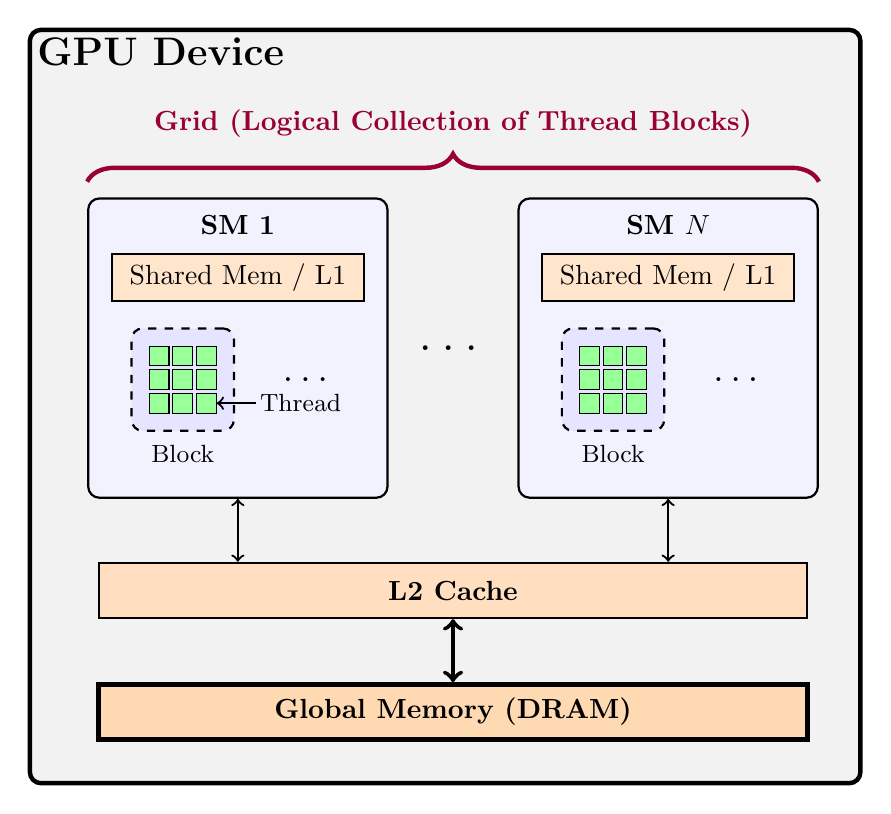
\begin{tikzpicture}[
        sm/.style={draw, thick, fill=blue!5, rounded corners, minimum width=3.8cm, minimum height=3.8cm},
        block/.style={draw, dashed, thick, fill=blue!10, rounded corners, inner sep=3pt},
        thread/.style={draw, fill=green!40, minimum width=0.25cm, minimum height=0.25cm, inner sep=0pt},
        mem/.style={draw, thick, fill=orange!20, minimum width=3.2cm, minimum height=0.6cm, align=center},
        l2/.style={draw, thick, fill=orange!25, minimum width=9cm, minimum height=0.7cm, align=center},
        gmem/.style={draw, ultra thick, fill=orange!30, minimum width=9cm, minimum height=0.7cm, align=center},
        device/.style={draw, ultra thick, fill=gray!10, rounded corners, inner sep=15pt}
    ]

    % SM 1
    \node[sm] (sm1) at (0,0) {};
    \node[anchor=north, font=\bfseries, yshift=-0.1cm] at (sm1.north) {SM 1};
    \node[mem, anchor=north, yshift=-0.7cm] (smem1) at (sm1.north) {Shared Mem / L1};

    % SM 1 - Block 1
    \node[block, minimum width=1.3cm, minimum height=1.3cm] (s1b1) at ($(sm1.center) + (-0.7, -0.4)$) {};
    \node[font=\small, anchor=north, yshift=-0.05cm] at (s1b1.south) {Block};
    \foreach \i/\x in {1/-0.3, 2/0, 3/0.3} {
        \foreach \j/\y in {1/0.3, 2/0, 3/-0.3} {
            \node[thread] (s1b1t\i\j) at ($(s1b1.center) + (\x, \y)$) {};
        }
    }

    % SM 1 - Multiple Blocks Dots
    \node[font=\Large] at ($(sm1.center) + (0.9, -0.4)$) {\dots};

    % Explicit annotation for Threads
    \draw[<-, thick] (s1b1t33.east) -- ++(0.5, 0) node[right, font=\small, inner sep=1pt] {Thread};

    % Dots indicating more SMs
    \node[right=0.25cm of sm1, font=\huge] (dots) {\dots};

    % SM N
    \node[sm, right=0.25cm of dots] (smn) {};
    \node[anchor=north, font=\bfseries, yshift=-0.1cm] at (smn.north) {SM $N$};
    \node[mem, anchor=north, yshift=-0.7cm] (smemn) at (smn.north) {Shared Mem / L1};

    % SM N - Block 1
    \node[block, minimum width=1.3cm, minimum height=1.3cm] (snb1) at ($(smn.center) + (-0.7, -0.4)$) {};
    \node[font=\small, anchor=north, yshift=-0.05cm] at (snb1.south) {Block};
    \foreach \i/\x in {1/-0.3, 2/0, 3/0.3} {
        \foreach \j/\y in {1/0.3, 2/0, 3/-0.3} {
            \node[thread] (snb1t\i\j) at ($(snb1.center) + (\x, \y)$) {};
        }
    }

    % SM N - Multiple Blocks Dots
    \node[font=\Large] at ($(smn.center) + (0.9, -0.4)$) {\dots};

    % Logical Grid Brace
    \draw[decorate, decoration={brace, amplitude=10pt}, ultra thick, purple!80!black]
        ([yshift=0.2cm]sm1.north west) -- ([yshift=0.2cm]smn.north east)
        node[midway, above=12pt, font=\bfseries, purple!80!black] {Grid (Logical Collection of Thread Blocks)};

    % L2 Cache (Centered between SM1 and SMN)
    \node[l2, anchor=north] (l2cache) at ($(sm1.south)!0.5!(smn.south) + (0, -0.8cm)$) {\textbf{L2 Cache}};

    % Global Memory
    \node[gmem, below=0.8cm of l2cache] (globalmem) {\textbf{Global Memory (DRAM)}};

    % Connections
    \draw[<->, thick] (sm1.south) -- (sm1.south |- l2cache.north);
    \draw[<->, thick] (smn.south) -- (smn.south |- l2cache.north);
    \draw[<->, ultra thick] (l2cache.south) -- (globalmem.north);

    % Device Background Layer
    \begin{scope}[on background layer]
        % Add a hidden coordinate to push the top border up slightly for the label and brace
        \coordinate (topleft) at ([xshift=-0.2cm, yshift=1.6cm]sm1.north west);
        \node[device, fit=(topleft) (smn) (globalmem)] (gpu) {};
        \node[anchor=north west, font=\Large\bfseries] at (gpu.north west) {GPU Device};
    \end{scope}

    \end{tikzpicture}}
    \caption{Schematic representation of a GPU architecture.}
    \label{fig:gpu_arch}
\end{figure}
The memory system is also hierarchical. Threads within an SM have access to fast on-chip storage, including registers and shared memory, which enables efficient intra-block cooperation and synchronization. SMs connect to a larger, device-wide cache (L2) and ultimately to high-capacity but high-latency global memory (DRAM). Effective GPU implementations therefore aim to expose ample parallelism while limiting expensive global-memory traffic \cite{nickolls2010gpu}.
This execution model is well suited for workloads dominated by large numbers of independent arithmetic operations and comparisons. In particular, pairwise dominance checks required during PF enumeration in Algorithm~\ref{alg:bidir_pf} are natural candidates for GPU acceleration.

\section{Implementation Details}
\label{app:implementation_details}

This appendix gives pseudocode for implementation details referenced in the main text but omitted there for space. The CPU detail is the pairwise reduction used to merge private cutset frontiers. The GPU details are the lower-level kernels used by Algorithm~\ref{alg:gpu_bidir_pf}.

\subsection{CPU Parallelization}
\label{app:cpu_implementation}

The CPU implementation uses the tree reduction in \Cref{alg:cpu_tree_reduction} to merge private cutset frontiers produced by different workers. This is the reduction referred to in \Cref{sec:cpu_impl}.

\begin{algorithm}[htbp]
\caption{CPU Tree Reduction for Cutset Frontiers}
\label{alg:cpu_tree_reduction}
\begin{algorithmic}[1]
\Require Private cutset frontiers $\mathcal{P} = [\mathcal{P}_1,\dots,\mathcal{P}_q]$
\Procedure{TreeReduce}{$\mathcal{P}$}
    \While{$|\mathcal{P}| > 1$}
        \State $\mathcal{Q} \gets [\,]$
        \ForAll{$i = 1,3,5,\dots,2\lfloor |\mathcal{P}|/2 \rfloor - 1$ \textbf{in parallel}}
            \State $\mathcal{Q}_{(i+1)/2} \gets \Call{FilterDominated}{\mathcal{P}_i \cup \mathcal{P}_{i+1}}$
        \EndFor
        \If{$|\mathcal{P}|$ is odd}
            \State $\mathcal{Q}_{\lfloor |\mathcal{P}|/2 \rfloor + 1} \gets \mathcal{P}_{|\mathcal{P}|}$
        \EndIf
        \State $\mathcal{P} \gets \mathcal{Q}$
    \EndWhile
    \State \Return $\mathcal{P}_1$
\EndProcedure
\end{algorithmic}
\end{algorithm}

\subsection{GPU Parallelization}
\label{app:gpu_implementation}

The GPU implementation expands each selected layer through the four-kernel pipeline described in \Cref{sec:gpu_impl}. \Cref{alg:compute_arc_offsets} computes per-arc candidate counts and buffer offsets. \Cref{alg:expand_candidates} then materializes shifted candidate labels in the assigned buffer segments. \Cref{alg:dynamic_1D_kernel} performs load-balanced dominance filtering, and \Cref{alg:compact_survivors} compacts the surviving labels into the next node-frontier representation. Finally, \Cref{alg:materialize_cutset_products} materializes the batched cutset products used by \textsc{Couple}$_{\mathrm{GPU}}$ in \Cref{alg:gpu_bidir_pf}.


\Cref{alg:expand_candidates} uses the offsets from \Cref{alg:compute_arc_offsets} to write every generated candidate into a disjoint location of the flat buffer.
\Cref{alg:dynamic_1D_kernel} assigns more thread blocks to nodes with larger candidate segments, so the dominance-filtering work is balanced at the level of node-frontier size.
\Cref{alg:compact_survivors} converts the binary survivor flags produced by the dominance kernel into compacted node-frontier storage.
\Cref{alg:materialize_cutset_products} is used during the batched cutset merge. It materializes the Cartesian products for a batch of active cutset nodes before filtering and merging them into the running global frontier.



\begin{algorithm}[t!]
\caption{Compute Candidate Offsets}
\label{alg:compute_arc_offsets}
\begin{algorithmic}[1]
\Require Frontier $\mathcal{Y}$; source-node array $b[]$; incoming-arc offsets $\phi^a[]$
\Procedure{ComputeArcOffsets}{$\mathcal{Y}, b, \phi^a$}
\State $M \gets |\mathcal{A}_{\mathcal{L}_j}|$ \Comment{Number of arcs in layer $j$}
\ForAll{arcs $a = 0$ \textbf{to} $M-1$ \textbf{in parallel on GPU}} \Comment{One thread per arc}
    \State $\kappa_a \gets |\mathcal{Y}(b(a))|$
\EndFor
\State $\phi^c_0 \gets 0$
\For{$a = 1$ \textbf{to} $M$ \textbf{in parallel on GPU}}
    \State $\phi^c_a \gets \phi^c_{a-1} + \kappa_{a-1}$
\EndFor
\ForAll{nodes $v \in \mathcal{L}_{j+1}$ \textbf{in parallel on GPU}}
    \State $a_{\text{first}} \gets \phi^a_v$
    \State $a_{\text{last}} \gets \phi^a_{v{+}1}$
    \State $\Gamma_v \gets \phi^c_{a_{\text{last}}} - \phi^c_{a_{\text{first}}}$
\EndFor
\State \Return $\kappa, \phi^c, \Gamma$
\EndProcedure
\end{algorithmic}
\end{algorithm}


\begin{algorithm}[htbp!]
\caption{Materialize Layer Candidates}
\label{alg:expand_candidates}
\begin{algorithmic}[1]
\Require Frontier $\mathcal{Y}$; source array $b[]$; arc weights $\mathbf{v}(\cdot)$; offsets $\phi^c[]$; counts $\kappa[]$
\Procedure{ExpandCandidates}{$\mathcal{Y}, b, \mathbf{v}, \phi^c, \kappa$}
\State Allocate flat buffer $\beta$ of size $\sum_a \kappa_a$
\ForAll{arcs $a$ \textbf{in parallel on GPU}}
    \State //~One warp (32 threads) per arc
    \ForAll{$k = 0, 1, \dots, \kappa_a{-}1$ \textbf{distributed across warp threads}}
        \State $\beta[\,\phi^c_a + k\,] \gets \mathcal{Y}(b(a))[k] + \mathbf{v}(a)$
    \EndFor
\EndFor
\State \Return $\beta$
\EndProcedure
\end{algorithmic}
\end{algorithm}


\begin{algorithm}[htbp!]
\caption{Compact Node Frontiers}
\label{alg:compact_survivors}
\begin{algorithmic}[1]
\Require Candidate buffer $\beta$ of size $S$; binary survivor flags $\sigma[]$
\Procedure{CompactSurvivors}{$\beta, \sigma$}
\State $\rho_0 \gets 0$
\For{$i = 1$ \textbf{to} $S$} \Comment{Parallel prefix sum on GPU}
    \State $\rho_i \gets \rho_{i-1} + \sigma_{i-1}$
\EndFor
\ForAll{candidates $i = 0$ \textbf{to} $S-1$ \textbf{in parallel on GPU}} \Comment{One thread per candidate}
    \If{$\sigma_i = 1$}
        \State $\mathcal{Y}(v)[\,\rho_i\,] \gets \beta[i]$ \Comment{$v$: destination node of $i$}
    \EndIf
\EndFor
\State \Return $\mathcal{Y}$
\EndProcedure
\end{algorithmic}
\end{algorithm}



\begin{algorithm}[htbp!]
\caption{Materialize Cutset Products}
\label{alg:materialize_cutset_products}
\begin{algorithmic}[1]
\Require Frontiers $\mathcal{Y}^{\downarrow}$, $\mathcal{Y}^{\uparrow}$; node offsets $\phi^{\downarrow}$, $\phi^{\uparrow}$ and sizes $\kappa^{\downarrow}$, $\kappa^{\uparrow}$ for nodes in batch $\mathcal{B}$; product offsets $\phi^p$
\Procedure{MaterializeProducts}{$\mathcal{Y}^{\downarrow}, \mathcal{Y}^{\uparrow}, \mathcal{B}$}
\State Allocate flat candidate buffer $\beta$ of size $\sum_{v \in \mathcal{B}} \kappa^{\downarrow}_v \cdot \kappa^{\uparrow}_v$
\ForAll{nodes $v \in \mathcal{B}$ \textbf{in parallel on GPU}} \Comment{One thread block per node}
    \State $T \gets \kappa^{\downarrow}_v \cdot \kappa^{\uparrow}_v$ \Comment{Total candidates for node $v$}
    \ForAll{candidate indices $p = 0, \dots, T-1$ \textbf{in parallel}}
        \State $i \gets \lfloor p / \kappa^{\uparrow}_v \rfloor$; \quad $j \gets p \pmod{\kappa^{\uparrow}_v}$
        \State $y^{\downarrow} \gets \mathcal{Y}^{\downarrow}(\phi^{\downarrow}_v + i)$; \quad $y^{\uparrow} \gets \mathcal{Y}^{\uparrow}(\phi^{\uparrow}_v + j)$
        \State $\beta[\,\phi^p_v + p\,] \gets y^{\downarrow} + y^{\uparrow}$
    \EndFor
\EndFor
\State \Return $\beta$
\EndProcedure
\end{algorithmic}
\end{algorithm}

\begin{algorithm}[t]
\caption{Load-Balanced GPU Dominance Filter}
\label{alg:dynamic_1D_kernel}
\begin{algorithmic}[1]
\Require Flat candidate buffer $\beta$; per-node candidate counts $\Gamma[]$; block size $B$
\Procedure{FilterDominated}{$\beta, \Gamma$}
\State $K[v] \gets \lceil \Gamma[v] / B \rceil$ for all $v$
\State $\phi^k_0 \gets 0$
\For{$v = 1$ \textbf{to} $|\mathcal{L}_{j+1}|$ \textbf{in parallel on GPU}}
    \State $\phi^k_v \gets \phi^k_{v-1} + K[v-1]$
\EndFor
\State $\sigma_i \gets 1$ for all candidates $i$
\ForAll{thread blocks $q = 0, \dots, \sum_v K[v] - 1$ \textbf{in parallel on GPU}}
    \State Binary search $\phi^k$ to find node $v$ s.t.\ $\phi^k_v \le q < \phi^k_{v{+}1}$
    \State $\tau \gets q - \phi^k_v$ \Comment{Tile index within node $v$}
    \State $[b,\, e) \gets$ candidate range of node $v$ in $\beta$
    \State $i \gets b + \tau \cdot B + \text{thread index within block}$
    \State \textbf{Load} $\mathbf{y}_i \gets \beta[i]$ into per-thread register (if $i < e$) \Comment{Reused across tiles}
    \State $\mathit{dominated} \gets \mathbf{false}$
    \For{tile start $s = b$ \textbf{to} $e{-}1$, \textbf{step} $B$}
        \State \textbf{Barrier}: wait for all threads in block
        \State Each thread $k$ loads $\beta[s{+}k]$ into \textbf{shared memory} slot $k$ \;(if $s{+}k < e$)
        \State \textbf{Barrier}: ensure tile is fully visible
        \If{$i < e$ \textbf{and not} $\mathit{dominated}$}
            \For{$j = 0$ \textbf{to} $\min(B,\, e{-}s){-}1$, \textbf{skip} $j = i{-}b{-}\tau B$}
                \If{shared[$j$] $\prec \mathbf{y}_i$}\; $\mathit{dominated} \gets \mathbf{true}$; \textbf{break} \EndIf
            \EndFor \Comment{Early exit within tile}
        \EndIf
        \If{$\mathit{dominated}$} \textbf{break} \EndIf \Comment{Early exit across tiles}
    \EndFor
    \If{$i < e$ \textbf{and} $\mathit{dominated}$}\; $\sigma_i \gets 0$ \EndIf
\EndFor
\State \Return $\sigma$
\EndProcedure
\end{algorithmic}
\end{algorithm}


\section{Additional Experimental Results}
\label{app:additional_results}

This appendix reports the full set of computational results summarized in \Cref{tab:combined_result_short}. The full MOKP, MOSPP, and MOTSP results are given in \Cref{tab:mokp_result,tab:mospp_result,tab:motsp_result}, respectively.

The complete MOKP runtime comparison is shown in \Cref{tab:mokp_result}. The complete MOSPP runtime comparison is shown in \Cref{tab:mospp_result}.

\begin{table*}[t]
\centering
\scriptsize
\caption{MOKP Pareto Enumeration Runtime Comparison Across Enumeration Methods}
\resizebox{0.8\textwidth}{!}{%
\begin{tabular}{rrlrrl|rrlrrl}
\toprule
N & K & Method & Time (S) & Speed-up & $S^{(M,T)}$ & N & K & Method & Time (S) & Speed-up & $S^{(M,T)}$ \\
\midrule
\multirow{8}{*}{40} & \multirow{8}{*}{6} & DPA-TS & 1371 & 0.01$\times$ & $2^{(0, 8)}$ & \multirow{8}{*}{40} & \multirow{8}{*}{7} & DPA-TS & -- & -- & $0^{(0, 10)}$ \\
 &  & DPA-A & 1439 & 0.01$\times$ & $2^{(0, 8)}$ &  &  & DPA-A & -- & -- & $0^{(0, 10)}$ \\
 &  & Coup & 10 & 1.00$\times$ & $10$ &  &  & Coup & 33 & 1.00$\times$ & $10$ \\
 &  & \texttt{Coup-4} & 6 & 1.87$\times$ & $10$ &  &  & \texttt{Coup-4} & 16 & 2.12$\times$ & $10$ \\
 &  & \texttt{Coup-8} & 5 & 2.15$\times$ & $10$ &  &  & \texttt{Coup-8} & 13 & 2.63$\times$ & $10$ \\
 &  & \texttt{Coup-16} & 4 & 2.60$\times$ & $10$ &  &  & \texttt{Coup-16} & 11 & 3.21$\times$ & $10$ \\
 &  & \texttt{G-TD} & 3 & 4.31$\times$ & $10$ &  &  & \texttt{G-TD} & 5 & 7.12$\times$ & $10$ \\
 &  & \texttt{G-Coup} & \textbf{2} & 5.51$\times$ & $10$ &  &  & \texttt{G-Coup} & \textbf{4} & 9.71$\times$ & $10$ \\
\midrule
\multirow{8}{*}{50} & \multirow{8}{*}{5} & DPA-TS & 1752 & 0.01$\times$ & $5^{(0, 5)}$ & \multirow{8}{*}{50} & \multirow{8}{*}{6} & DPA-TS & -- & -- & $0^{(0, 10)}$ \\
 &  & DPA-A & 1625 & 0.01$\times$ & $5^{(0, 5)}$ &  &  & DPA-A & -- & -- & $0^{(0, 10)}$ \\
 &  & Coup & 19 & 1.00$\times$ & $10$ &  &  & Coup & 184 & 1.00$\times$ & $10$ \\
 &  & \texttt{Coup-4} & 9 & 2.06$\times$ & $10$ &  &  & \texttt{Coup-4} & 82 & 2.26$\times$ & $10$ \\
 &  & \texttt{Coup-8} & 8 & 2.42$\times$ & $10$ &  &  & \texttt{Coup-8} & 63 & 2.94$\times$ & $10$ \\
 &  & \texttt{Coup-16} & 7 & 2.93$\times$ & $10$ &  &  & \texttt{Coup-16} & 52 & 3.59$\times$ & $10$ \\
 &  & \texttt{G-TD} & \textbf{3} & 6.49$\times$ & $10$ &  &  & \texttt{G-TD} & 45 & 4.09$\times$ & $10$ \\
 &  & \texttt{G-Coup} & 4 & 5.89$\times$ & $10$ &  &  & \texttt{G-Coup} & \textbf{26} & 7.12$\times$ & $10$ \\
\midrule
\multirow{8}{*}{50} & \multirow{8}{*}{7} & DPA-TS & -- & -- & $0^{(0, 10)}$ & \multirow{8}{*}{60} & \multirow{8}{*}{4} & DPA-TS & 1102 & 0.01$\times$ & $9^{(0, 1)}$ \\
 &  & DPA-A & -- & -- & $0^{(0, 10)}$ &  &  & DPA-A & 925 & 0.02$\times$ & $9^{(0, 1)}$ \\
 &  & Coup & 499 & 1.00$\times$ & $10$ &  &  & Coup & 16 & 1.00$\times$ & $10$ \\
 &  & \texttt{Coup-4} & 229 & 2.18$\times$ & $10$ &  &  & \texttt{Coup-4} & 8 & 2.04$\times$ & $10$ \\
 &  & \texttt{Coup-8} & 180 & 2.78$\times$ & $10$ &  &  & \texttt{Coup-8} & 7 & 2.36$\times$ & $10$ \\
 &  & \texttt{Coup-16} & 150 & 3.34$\times$ & $10$ &  &  & \texttt{Coup-16} & 6 & 3.01$\times$ & $10$ \\
 &  & \texttt{G-TD} & \textbf{81} & 6.20$\times$ & $10$ &  &  & \texttt{G-TD} & \textbf{3} & 7.74$\times$ & $10$ \\
 &  & \texttt{G-Coup} & 82 & 6.08$\times$ & $10$ &  &  & \texttt{G-Coup} & 3 & 6.98$\times$ & $10$ \\
\midrule
\multirow{8}{*}{60} & \multirow{8}{*}{5} & DPA-TS & -- & -- & $0^{(0, 10)}$ & \multirow{8}{*}{60} & \multirow{8}{*}{6} & DPA-TS & -- & -- & $0^{(0, 10)}$ \\
 &  & DPA-A & -- & -- & $0^{(0, 10)}$ &  &  & DPA-A & -- & -- & $0^{(0, 10)}$ \\
 &  & Coup & 190 & 1.00$\times$ & $10$ &  &  & Coup & 849 & 1.00$\times$ & $8^{(0, 2)}$ \\
 &  & \texttt{Coup-4} & 84 & 2.27$\times$ & $10$ &  &  & \texttt{Coup-4} & 678 & 1.25$\times$ & $10$ \\
 &  & \texttt{Coup-8} & 67 & 2.83$\times$ & $10$ &  &  & \texttt{Coup-8} & 424 & 2.00$\times$ & $10$ \\
 &  & \texttt{Coup-16} & 57 & 3.34$\times$ & $10$ &  &  & \texttt{Coup-16} & 341 & 2.49$\times$ & $10$ \\
 &  & \texttt{G-TD} & \textbf{30} & 6.31$\times$ & $10$ &  &  & \texttt{G-TD} & 201 & 4.23$\times$ & $10$ \\
 &  & \texttt{G-Coup} & 30 & 6.31$\times$ & $10$ &  &  & \texttt{G-Coup} & \textbf{156} & 5.45$\times$ & $10$ \\
\midrule
\multirow{8}{*}{60} & \multirow{8}{*}{7} & DPA-TS & -- & -- & $0^{(0, 10)}$ & \multirow{8}{*}{70} & \multirow{8}{*}{3} & DPA-TS & 87 & 0.05$\times$ & $10$ \\
 &  & DPA-A & -- & -- & $0^{(0, 10)}$ &  &  & DPA-A & 62 & 0.07$\times$ & $10$ \\
 &  & Coup & 1244 & 1.00$\times$ & $6^{(0, 4)}$ &  &  & Coup & 5 & 1.00$\times$ & $10$ \\
 &  & \texttt{Coup-4} & 969 & 1.28$\times$ & $7^{(0, 3)}$ &  &  & \texttt{Coup-4} & 3 & 1.61$\times$ & $10$ \\
 &  & \texttt{Coup-8} & 730 & 1.71$\times$ & $7^{(0, 3)}$ &  &  & \texttt{Coup-8} & 3 & 1.61$\times$ & $10$ \\
 &  & \texttt{Coup-16} & 607 & 2.05$\times$ & $7^{(0, 3)}$ &  &  & \texttt{Coup-16} & 3 & 1.80$\times$ & $10$ \\
 &  & \texttt{G-TD} & \textbf{325} & 3.83$\times$ & $6^{(4, 0)}$ &  &  & \texttt{G-TD} & \textbf{2} & 3.38$\times$ & $10$ \\
 &  & \texttt{G-Coup} & 787 & 1.58$\times$ & $10$ &  &  & \texttt{G-Coup} & 2 & 2.78$\times$ & $10$ \\
\midrule
\multirow{8}{*}{70} & \multirow{8}{*}{4} & DPA-TS & 2144 & 0.03$\times$ & $6^{(0, 4)}$ & \multirow{8}{*}{70} & \multirow{8}{*}{5} & DPA-TS & -- & -- & $0^{(0, 10)}$ \\
 &  & DPA-A & 2130 & 0.03$\times$ & $7^{(0, 3)}$ &  &  & DPA-A & -- & -- & $0^{(0, 10)}$ \\
 &  & Coup & 70 & 1.00$\times$ & $10$ &  &  & Coup & 768 & 1.00$\times$ & $8^{(0, 2)}$ \\
 &  & \texttt{Coup-4} & 33 & 2.12$\times$ & $10$ &  &  & \texttt{Coup-4} & 728 & 1.05$\times$ & $9^{(0, 1)}$ \\
 &  & \texttt{Coup-8} & 27 & 2.64$\times$ & $10$ &  &  & \texttt{Coup-8} & 539 & 1.42$\times$ & $9^{(0, 1)}$ \\
 &  & \texttt{Coup-16} & 23 & 3.08$\times$ & $10$ &  &  & \texttt{Coup-16} & 649 & 1.18$\times$ & $10$ \\
 &  & \texttt{G-TD} & \textbf{9} & 8.41$\times$ & $10$ &  &  & \texttt{G-TD} & \textbf{182} & 4.22$\times$ & $9^{(1, 0)}$ \\
 &  & \texttt{G-Coup} & 9 & 8.28$\times$ & $10$ &  &  & \texttt{G-Coup} & 291 & 2.64$\times$ & $10$ \\
\midrule
\multirow{8}{*}{70} & \multirow{8}{*}{6} & DPA-TS & -- & -- & $0^{(0, 10)}$ & \multirow{8}{*}{70} & \multirow{8}{*}{7} & DPA-TS & -- & -- & $0^{(0, 10)}$ \\
 &  & DPA-A & -- & -- & $0^{(0, 10)}$ &  &  & DPA-A & -- & -- & $0^{(0, 10)}$ \\
 &  & Coup & 1549 & 1.00$\times$ & $5^{(0, 5)}$ &  &  & Coup & 1650 & 1.00$\times$ & $3^{(0, 7)}$ \\
 &  & \texttt{Coup-4} & 1326 & 1.17$\times$ & $7^{(0, 3)}$ &  &  & \texttt{Coup-4} & 1391 & 1.19$\times$ & $4^{(0, 6)}$ \\
 &  & \texttt{Coup-8} & 1008 & 1.54$\times$ & $7^{(0, 3)}$ &  &  & \texttt{Coup-8} & 1757 & 0.94$\times$ & $6^{(0, 4)}$ \\
 &  & \texttt{Coup-16} & 862 & 1.80$\times$ & $7^{(0, 3)}$ &  &  & \texttt{Coup-16} & 1708 & 0.97$\times$ & $7^{(0, 3)}$ \\
 &  & \texttt{G-TD} & \textbf{335} & 4.63$\times$ & $6^{(4, 0)}$ &  &  & \texttt{G-TD} & \textbf{372} & 4.44$\times$ & $3^{(7, 0)}$ \\
 &  & \texttt{G-Coup} & 1010 & 1.53$\times$ & $10$ &  &  & \texttt{G-Coup} & 907 & 1.82$\times$ & $6^{(3, 1)}$ \\
\bottomrule
\end{tabular}
}
\label{tab:mokp_result}
\end{table*}

\begin{table*}[t]
\centering
\scriptsize
\caption{MOSPP Pareto Enumeration Runtime Comparison Across Enumeration Methods}
\resizebox{0.8\textwidth}{!}{%
\begin{tabular}{rrlrrl|rrlrrl}
\toprule
N & K & Method & Time (S) & Speed-up & $S^{(M,T)}$ & N & K & Method & Time (S) & Speed-up & $S^{(M,T)}$ \\
\midrule
\multirow{8}{*}{150} & \multirow{8}{*}{3} & DPA-TS & 11 & 1.12$\times$ & $10$ & \multirow{8}{*}{150} & \multirow{8}{*}{4} & DPA-TS & 486 & 0.03$\times$ & $10$ \\
 &  & DPA-A & 8 & 1.59$\times$ & $10$ &  &  & DPA-A & 420 & 0.04$\times$ & $10$ \\
 &  & Coup & 12 & 1.00$\times$ & $10$ &  &  & Coup & 16 & 1.00$\times$ & $10$ \\
 &  & \texttt{Coup-4} & 8 & 1.50$\times$ & $10$ &  &  & \texttt{Coup-4} & 10 & 1.54$\times$ & $10$ \\
 &  & \texttt{Coup-8} & 8 & 1.50$\times$ & $10$ &  &  & \texttt{Coup-8} & 9 & 1.84$\times$ & $10$ \\
 &  & \texttt{Coup-16} & 8 & 1.51$\times$ & $10$ &  &  & \texttt{Coup-16} & 7 & 2.16$\times$ & $10$ \\
 &  & \texttt{G-TD} & 7 & 1.80$\times$ & $10$ &  &  & \texttt{G-TD} & 6 & 2.74$\times$ & $10$ \\
 &  & \texttt{G-Coup} & \textbf{5} & 2.44$\times$ & $9^{(1, 0)}$ &  &  & \texttt{G-Coup} & \textbf{6} & 2.94$\times$ & $9^{(1, 0)}$ \\
\midrule
\multirow{8}{*}{150} & \multirow{8}{*}{5} & DPA-TS & 1929 & 0.02$\times$ & $5^{(0, 5)}$ & \multirow{8}{*}{150} & \multirow{8}{*}{6} & DPA-TS & 1052 & 0.04$\times$ & $1^{(0, 9)}$ \\
 &  & DPA-A & 1807 & 0.02$\times$ & $5^{(0, 5)}$ &  &  & DPA-A & 1085 & 0.04$\times$ & $1^{(0, 9)}$ \\
 &  & Coup & 34 & 1.00$\times$ & $10$ &  &  & Coup & 47 & 1.00$\times$ & $10$ \\
 &  & \texttt{Coup-4} & 20 & 1.72$\times$ & $10$ &  &  & \texttt{Coup-4} & 26 & 1.86$\times$ & $10$ \\
 &  & \texttt{Coup-8} & 18 & 1.89$\times$ & $10$ &  &  & \texttt{Coup-8} & 22 & 2.16$\times$ & $10$ \\
 &  & \texttt{Coup-16} & 16 & 2.11$\times$ & $10$ &  &  & \texttt{Coup-16} & 21 & 2.32$\times$ & $10$ \\
 &  & \texttt{G-TD} & \textbf{10} & 3.35$\times$ & $10$ &  &  & \texttt{G-TD} & \textbf{6} & 8.42$\times$ & $10$ \\
 &  & \texttt{G-Coup} & 11 & 3.17$\times$ & $10$ &  &  & \texttt{G-Coup} & 7 & 6.76$\times$ & $10$ \\
\midrule
\multirow{8}{*}{150} & \multirow{8}{*}{7} & DPA-TS & -- & -- & $0^{(0, 10)}$ & \multirow{8}{*}{200} & \multirow{8}{*}{3} & DPA-TS & 32 & 5.15$\times$ & $10$ \\
 &  & DPA-A & -- & -- & $0^{(0, 10)}$ &  &  & DPA-A & \textbf{22} & 7.53$\times$ & $10$ \\
 &  & Coup & 184 & 1.00$\times$ & $10$ &  &  & Coup & 162 & 1.00$\times$ & $1^{(9, 0)}$ \\
 &  & \texttt{Coup-4} & 84 & 2.20$\times$ & $10$ &  &  & \texttt{Coup-4} & 93 & 1.75$\times$ & $1^{(9, 0)}$ \\
 &  & \texttt{Coup-8} & 71 & 2.61$\times$ & $10$ &  &  & \texttt{Coup-8} & 87 & 1.86$\times$ & $1^{(9, 0)}$ \\
 &  & \texttt{Coup-16} & 96 & 1.91$\times$ & $10$ &  &  & \texttt{Coup-16} & 72 & 2.27$\times$ & $1^{(8, 1)}$ \\
 &  & \texttt{G-TD} & \textbf{9} & 20.88$\times$ & $10$ &  &  & \texttt{G-TD} & -- & -- & $0^{(10, 0)}$ \\
 &  & \texttt{G-Coup} & 17 & 10.98$\times$ & $10$ &  &  & \texttt{G-Coup} & -- & -- & $0^{(10, 0)}$ \\
\midrule
\multirow{8}{*}{200} & \multirow{8}{*}{4} & DPA-TS & 913 & 0.20$\times$ & $10$ &  &  &  &  &  &  \\
 &  & DPA-A & 793 & 0.23$\times$ & $10$ &  &  &  &  &  &  \\
 &  & Coup & 186 & 1.00$\times$ & $1^{(9, 0)}$ &  &  &  &  &  &  \\
 &  & \texttt{Coup-4} & 80 & 2.34$\times$ & $1^{(9, 0)}$ &  &  &  &  &  &  \\
 &  & \texttt{Coup-8} & 63 & 2.97$\times$ & $1^{(9, 0)}$ &  &  &  &  &  &  \\
 &  & \texttt{Coup-16} & \textbf{45} & 4.12$\times$ & $1^{(9, 0)}$ &  &  &  &  &  &  \\
 &  & \texttt{G-TD} & -- & -- & $0^{(10, 0)}$ &  &  &  &  &  &  \\
 &  & \texttt{G-Coup} & -- & -- & $0^{(10, 0)}$ &  &  &  &  &  &  \\
\bottomrule
\end{tabular}
}
\label{tab:mospp_result}
\end{table*}

The complete MOTSP runtime comparison is shown in \Cref{tab:motsp_result}.
\begin{table*}[t]
\centering
\scriptsize
\caption{MOTSP Pareto Enumeration Runtime Comparison Across Enumeration Methods}
\resizebox{0.8\textwidth}{!}{%
\begin{tabular}{rrlrrl|rrlrrl}
\toprule
N & K & Method & Time (S) & Speed-up & $S^{(M,T)}$ & N & K & Method & Time (S) & Speed-up & $S^{(M,T)}$ \\
\midrule
\multirow{8}{*}{15} & \multirow{8}{*}{4} & DPA-TS & -- & -- & $0^{(0, 10)}$ & \multirow{8}{*}{15} & \multirow{8}{*}{5} & DPA-TS & -- & -- & $0^{(0, 10)}$ \\
 &  & DPA-A & -- & -- & $0^{(0, 10)}$ &  &  & DPA-A & -- & -- & $0^{(0, 10)}$ \\
 &  & Coup & 23 & 1.00$\times$ & $10$ &  &  & Coup & 335 & 1.00$\times$ & $10$ \\
 &  & \texttt{Coup-4} & 7 & 3.47$\times$ & $10$ &  &  & \texttt{Coup-4} & 115 & 2.92$\times$ & $10$ \\
 &  & \texttt{Coup-8} & 5 & 5.06$\times$ & $10$ &  &  & \texttt{Coup-8} & 82 & 4.11$\times$ & $10$ \\
 &  & \texttt{Coup-16} & 3 & 7.83$\times$ & $10$ &  &  & \texttt{Coup-16} & 67 & 5.05$\times$ & $10$ \\
 &  & \texttt{G-TD} & 3 & 7.50$\times$ & $10$ &  &  & \texttt{G-TD} & \textbf{36} & 9.44$\times$ & $9^{(1, 0)}$ \\
 &  & \texttt{G-Coup} & \textbf{3} & 8.03$\times$ & $10$ &  &  & \texttt{G-Coup} & 48 & 7.04$\times$ & $10$ \\
\midrule
\multirow{8}{*}{15} & \multirow{8}{*}{6} & DPA-TS & -- & -- & $0^{(0, 10)}$ & \multirow{8}{*}{15} & \multirow{8}{*}{7} & DPA-TS & -- & -- & $0^{(0, 10)}$ \\
 &  & DPA-A & -- & -- & $0^{(0, 10)}$ &  &  & DPA-A & -- & -- & $0^{(0, 10)}$ \\
 &  & Coup & 1623 & 1.00$\times$ & $9^{(0, 1)}$ &  &  & Coup & 3544 & 1.00$\times$ & $1^{(0, 9)}$ \\
 &  & \texttt{Coup-4} & 870 & 1.87$\times$ & $10$ &  &  & \texttt{Coup-4} & 2508 & 1.41$\times$ & $3^{(0, 7)}$ \\
 &  & \texttt{Coup-8} & 711 & 2.28$\times$ & $10$ &  &  & \texttt{Coup-8} & 2123 & 1.67$\times$ & $3^{(0, 7)}$ \\
 &  & \texttt{Coup-16} & 641 & 2.53$\times$ & $10$ &  &  & \texttt{Coup-16} & 1930 & 1.84$\times$ & $3^{(0, 7)}$ \\
 &  & \texttt{G-TD} & -- & -- & $0^{(10, 0)}$ &  &  & \texttt{G-TD} & -- & -- & $0^{(10, 0)}$ \\
 &  & \texttt{G-Coup} & \textbf{369} & 4.40$\times$ & $10$ &  &  & \texttt{G-Coup} & \textbf{1828} & 1.94$\times$ & $6^{(3, 1)}$ \\
\bottomrule
\end{tabular}
}
\label{tab:motsp_result}
\end{table*}



\end{document}
